\documentclass[conference]{IEEEtran}
\IEEEoverridecommandlockouts
% The preceding line is only needed to identify funding in the first footnote. If that is unneeded, please comment it out.
\usepackage{cite}
\usepackage{amsmath,amssymb,amsfonts}
\usepackage{algorithmic}
\usepackage{graphicx}
\usepackage{textcomp}
\usepackage{xcolor}
\usepackage{tikz}
\def\BibTeX{{\rm B\kern-.05em{\sc i\kern-.025em b}\kern-.08em
    T\kern-.1667em\lower.7ex\hbox{E}\kern-.125emX}}
\begin{document}

\title{Ceng435 Term Project Part1\\
}

\author{\IEEEauthorblockN{Mert Anıl YILMAZ}
\IEEEauthorblockA{\textit{Group 84} \\
2172211 \\
e2172211@ceng.metu.edu.tr}
\and
\IEEEauthorblockN{Onur Can ÜNAL}
\IEEEauthorblockA{\textit{Group 84} \\
2095966 \\
e2095966@ceng.metu.edu.tr}
}

\maketitle

\section{Abstract}
The project is aimed to reduce the end-to-end delay by finding the shortest path between source and destination for a network case that there are 5 nodes including source and destination and to do three experiments with different delays so that plotting network emulation delay vs. end-to-end delay graph with a 95$\%$ confidence interval for each of the different communication. In this project, packets are sent as datagrams by using UDP (User Datagram Protocol) which is a transport layer protocol.
\section{Design and Implementation Approach}
First of all, we used GENI Platform in order to obtain sources. We had some problems when allocating the sources, so we repeated this phases a lot. After we got the sources, we upload our default xml file in order to obtain the topology that were given. After that, we configured r1 and r2 nodes by using configureR1.sh and configureR2.sh, respectively. After that, our topology is ready to use.
\subsection{Scenarios}
In our topology, we have 5 nodes. 3 of these are router nodes and the other nodes are source and destination. Since we need to calculate link costs, Round Trip Time (RTT) values, we need a scenario that guarantees that there is no duplicate calculation for each link. Therefore, we designed our scenario with one way links. \\

Normally, we aim to send a packet from source to destination. Therefore, we could choose a scenario like this: s-$>$r2-$>$... However, if we did like this, we could encounter a problem. RTT is the one complete tour including request and response of a packet between two nodes. However, in the project, we have to pick all RTT values in router nodes. It means that since this route leads us to obtain RTT value in s node, we have to send one more packet to r2 and the packet will include RTT value of the node. Since we want to eliminate this extra packet, we chose the scenarios like this: r2-$>$s, r1-$>$d ... \\

\begin{center}
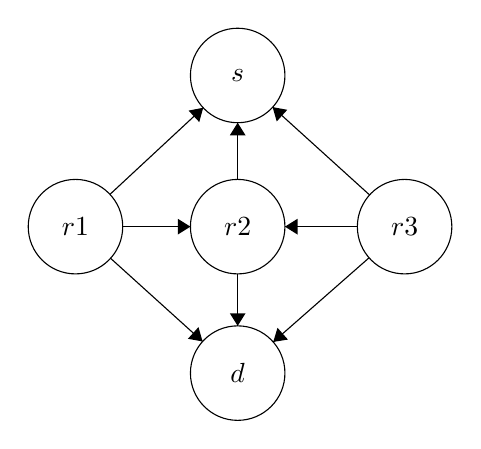
\begin{tikzpicture}[scale=0.2]
\tikzstyle{every node}+=[inner sep=0pt]
\draw [black] (37.3,-9.3) circle (3);
\draw (37.3,-9.3) node {$s$};
\draw [black] (37.3,-28.2) circle (3);
\draw (37.3,-28.2) node {$d$};
\draw [black] (47.9,-18.9) circle (3);
\draw (47.9,-18.9) node {$r3$};
\draw [black] (27,-18.9) circle (3);
\draw (27,-18.9) node {$r1$};
\draw [black] (37.3,-18.9) circle (3);
\draw (37.3,-18.9) node {$r2$};
\draw [black] (45.64,-20.88) -- (39.56,-26.22);
\fill [black] (39.56,-26.22) -- (40.49,-26.07) -- (39.83,-25.32);
\draw [black] (37.3,-21.9) -- (37.3,-25.2);
\fill [black] (37.3,-25.2) -- (37.8,-24.4) -- (36.8,-24.4);
\draw [black] (29.23,-20.91) -- (35.07,-26.19);
\fill [black] (35.07,-26.19) -- (34.81,-25.28) -- (34.14,-26.02);
\draw [black] (44.9,-18.9) -- (40.3,-18.9);
\fill [black] (40.3,-18.9) -- (41.1,-19.4) -- (41.1,-18.4);
\draw [black] (30,-18.9) -- (34.3,-18.9);
\fill [black] (34.3,-18.9) -- (33.5,-18.4) -- (33.5,-19.4);
\draw [black] (29.19,-16.85) -- (35.11,-11.35);
\fill [black] (35.11,-11.35) -- (34.18,-11.53) -- (34.86,-12.26);
\draw [black] (37.3,-15.9) -- (37.3,-12.3);
\fill [black] (37.3,-12.3) -- (36.8,-13.1) -- (37.8,-13.1);
\draw [black] (45.68,-16.89) -- (39.52,-11.31);
\fill [black] (39.52,-11.31) -- (39.78,-12.22) -- (40.45,-11.48);
\end{tikzpicture}
\end{center}

The complete approach of our scenarios can be seen above. In this design, we hold the start time, when a packet sends, and after the response returns, we hold the finish time and we simply subtract these two time values to calculate RTT of the corresponding link. The other advantage of this design is that we do not have time synchronization problem because we hold both time values in the same node. \\

\subsection{Link Costs}
In this design, both r1 and r3 send packets to s, r2, and d and take the responses of these packets in order to calculate RTT values. s and d are responsible for sending response to the corresponding node for the each packet. It means that, in the first part of the project, link cost calculations, both s and d nodes act as a destination node. Apart from these, r2 has to have methods both sending a packet and receiving a packet. \\

We determined buffer size as 1000 and we decided to send 1000 packets in order to obtain more accurate values for RTT for each link. After that, we simply take the average of these. \\

Our outcomes were interesting, because we noticed that the reason why we had configureR1.sh and configureR2.sh. When we setup our topology, we simply followed the instructions and we did not looked at the content of these .sh files. After we obtained RTT values, we noticed that the links which are connected to r1 and r2 are more costly. After we looked at the content of the .sh files, we noticed that we added random delays to these links. \\ \\ \\

Our r1, r2, and r3 scripts create txt files listing all link costs. The link costs are below. All costs are calculated as second, not millisecond. \\ \\
d-r1: 0.060889182567596435 \\
s-r1: 0.06089199328422546 \\
r1-r2: 0.1408923192024231 \\
s-r2: 0.08089756035804749 \\
d-r2: 0.080899489402771 \\
s-r3: 0.0003198683261871338 \\
d-r3: 0.0003284502029418945 \\
r2-r3: 0.08082268571853637 \\

\subsection{UDP and Multi-threding}
All nodes will implement a client/server application that sends and receives multiple messages at the same time, we need to a asynchronous design approach. Therefore, our scripts have to run multiple threads at the same time. We achieved this by using threading library. We simply created threads in each script by calling our functions, client and server. We determined the number of threads by looking at the degree of nodes. For example, since r1 has three connected links, its degree is three. When we created these threads, we had to be very careful because each nodes have different IPs for each link. We had to give the right IP for each client threads. \\

Our UDP implementation is simple. We have basically two functions which are named client and server. There are some similarities and some differences for these functions. We have to create a socket instance for each function in order to communicate each other. The transport layer protocol is specified as a parameter of the socket instance. We specified UDP as transport layer protocol. First of all, we are not sure whether our all packets reach the destination node because there is no control mechanism for UDP. We took lots of trials and we obtained 1000 responses for each 1000 request. In spite of that, we used a counter to guarantee that average of RTTs are calculated correctly even there is a packet loss. While client function has IP and the port number of destination, server function specifies the port and waits to take the discovery messages. \\

\subsection{Finding the Shortest Path using the Dijkstra Algorithm}


\begin{figure}[htp]
    \centering
    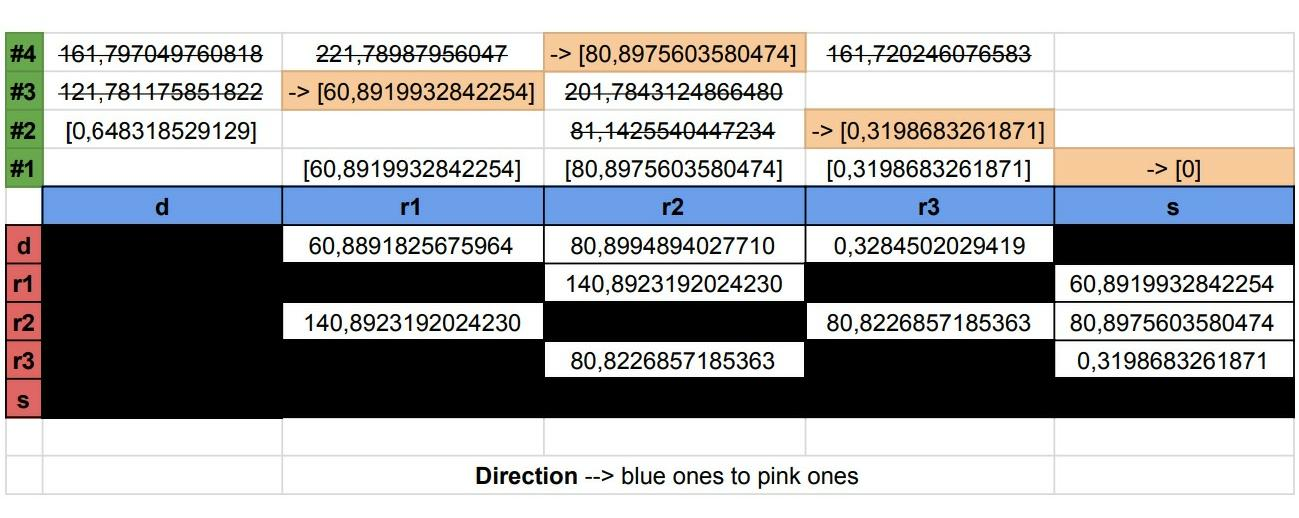
\includegraphics[width=9cm]{dijkstra.jpeg}
    \caption{Dijkstra Algorithm displaying on the table}
    \label{fig:dijkstra}
\end{figure}

We used the table representation of Dijkstra Algorithm shown in Figure 1 when calculating the shortest path. First of all, we prepared the table which includes link costs between nodes. The important point is that we prepared the table according to all available paths. The transmission ways are can be represented as tuple such as (node1, node2). node1 demonstrates sender node, and node2 demonstrates receiver node. It is demonstrated in the table the way that blue rows represent node1s and the pink column represent node2s. Since all combinations are not available or redundant, some entries of the table are showed as a black box. For example, since there is no link between r1 and r3, both (r1,r3) and (r3,r1) entries are shown as a black box. Since returning back to previous node only increases the cost, for any shortest path algorithm, this will be meaningless. Therefore, for example, (r1,s) tuple is shown as a black box, too. Moreover, all (i,j)s where i=j are shown as black box. \\

To be more clear, we demonstrates all available paths below as a graph, too. \\

\begin{center}
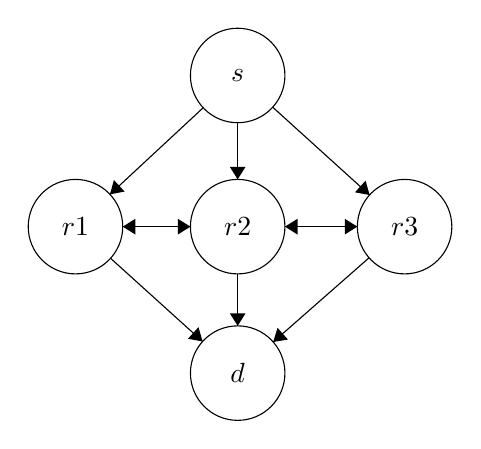
\begin{tikzpicture}[scale=0.2]
\tikzstyle{every node}+=[inner sep=0pt]
\draw [black] (37.3,-9.3) circle (3);
\draw (37.3,-9.3) node {$s$};
\draw [black] (37.3,-28.2) circle (3);
\draw (37.3,-28.2) node {$d$};
\draw [black] (47.9,-18.9) circle (3);
\draw (47.9,-18.9) node {$r3$};
\draw [black] (27,-18.9) circle (3);
\draw (27,-18.9) node {$r1$};
\draw [black] (37.3,-18.9) circle (3);
\draw (37.3,-18.9) node {$r2$};
\draw [black] (45.64,-20.88) -- (39.56,-26.22);
\fill [black] (39.56,-26.22) -- (40.49,-26.07) -- (39.83,-25.32);
\draw [black] (37.3,-21.9) -- (37.3,-25.2);
\fill [black] (37.3,-25.2) -- (37.8,-24.4) -- (36.8,-24.4);
\draw [black] (29.23,-20.91) -- (35.07,-26.19);
\fill [black] (35.07,-26.19) -- (34.81,-25.28) -- (34.14,-26.02);
\draw [black] (30,-18.9) -- (34.3,-18.9);
\fill [black] (34.3,-18.9) -- (33.5,-18.4) -- (33.5,-19.4);
\draw [black] (44.9,-18.9) -- (40.3,-18.9);
\fill [black] (40.3,-18.9) -- (41.1,-19.4) -- (41.1,-18.4);
\draw [black] (35.11,-11.35) -- (29.19,-16.85);
\fill [black] (29.19,-16.85) -- (30.12,-16.67) -- (29.44,-15.94);
\draw [black] (37.3,-12.3) -- (37.3,-15.9);
\fill [black] (37.3,-15.9) -- (37.8,-15.1) -- (36.8,-15.1);
\draw [black] (39.52,-11.31) -- (45.68,-16.89);
\fill [black] (45.68,-16.89) -- (45.42,-15.98) -- (44.75,-16.72);
\draw [black] (34.3,-18.9) -- (30,-18.9);
\fill [black] (30,-18.9) -- (30.8,-19.4) -- (30.8,-18.4);
\draw [black] (40.3,-18.9) -- (44.9,-18.9);
\fill [black] (44.9,-18.9) -- (44.1,-18.4) -- (44.1,-19.4);
\end{tikzpicture}
\end{center}

We found the shortest path with 4 iterations in this table representation. All iterations are shown on the table and the iteration numbers are shown with green column.\\

$\bold{Iteration}$ $\bold{1:}$ \\

Since we aimed to send packets from source to destination, we need to find the shortest path between these. Therefore, our initial node will be s in this algorithm. We set the initial cost as 0 and we add link costs to initial cost and we write the result in the corresponding node's table entry. For example, 60.8919932842254 ms is the cost link for s-r1. We add this cost to initial cost of s, 0 and we write it above the blue entry of r1. We do similar calculations for r2 and r3, too. \\

$\bold{Iteration}$ $\bold{2:}$ \\

We look at the cost to arrive router nodes from source and we choose the node which has smallest cost. In previous iteration, s is the chosen node while in this iteration, r3 is the chosen node. We look at possible links and we add the cost to arrive r3 from s and the link costs of possible links and we aim to update the costs if the new costs of nodes are smaller than previous one. However, the new cost of r2 is bigger than previous one, therefore we simply cross out the new cost, 81.1425540447234 ms. Since d has no cost from the first iteration, we simlpy write the new cost of arriving d, 0.648318529129 in the entry. \\

$\bold{Iteration}$ $\bold{3}$ $\bold{and}$ $\bold{4:}$ \\

We choose a new node which has smallest cost among not chosen nodes before. After that, we repeated the algorithm in these iterations. After these iterations, the shortest path does not change. The cost of the path s--$> $r3--$> $d is the smallest cost to arrive d from s. \\

\section{Methodology}

We chose Python as programming language since our lecture book presented socket programming with Python and explained that Python is easy to use for socket programming: "... we chose Python mostly because Python clearly exposes the key socket concepts. With Python there are fewer lines of code, and each line can be explained to the novice programmer without difficulty." \\

In addition to Python, we used some libraries which are threading, time and socket. threading library is for obtaining asynchronous threads. time library is for delay calculations and socket library is for building network. \\

\section{Motivation}

Since we are not familiar with socket programming which is included in almost every new technology product, we are willing to learn this concept by doing this project. In addition to it, we experienced the importance of minimizing the delay. We had a chance to use our theoretical knowledge about protocols in this project. Apart from those, the project's content is parallel with our aim in the other course, CEng491. We will try to provide better connection for each subscriber in our CEng491 project. \\

\section{Experiments}

For this part for the Term Project, we had to change our scripts which we prepared for previous parts. For the calculation of link costs, we used a logic such that r1, r2, and r3 nodes send, and s and d nodes take. While there were server programs on s and d, there were clients programs on nodes r1 and r3, and there were both client and server programs on node r2. On the other hand, for this part, there should be a client program on node s, there should be both client and server programs on node r3, and there should be a server program on node d.  \\

After we examined configureR1.sh and configureR2.sh, we prepared 12 configuration files in total. We have three nodes, s, d, and r3 to configure and we have three experiments. Therefore, actually, 9 configuration files were enough but we wanted to tested our scripts with 0 emulation delay. Therefore, there are one more configuration file for each three nodes. We did small changes in configureR1.sh and we obtained new configuration files easily. We used our experiment delays, for instance 20 ms +/- 5 ms, instead of random delays. \\

As we found the shortest path as s - r3 - d path, we used this path to send packets. Since we used UDP as protocol, there can be loss of packets. Thus, we chose higher number of packets (5000) to send so that we could get more reliable results. By this way, although the number of packets that node d receives can change, it is always higher and more reliable since we need average end-to-end delays and standard deviation. \\

We thought to start to calculate end-to-end delays without any network emulation delay, firstly. We implemented node s as a client. It sends 5000 packets to get more accurate results in case of many packet loss. While we were sending packets, we though to use '-' character as the terminating character to acknowledge that sending packets is over. When r3 node gets a '-' character, it ends receiving packets. Since there is a probability to loss the terminating packet, we sent 100 identical terminating packets to have more reliable design. \\

In calculating the link costs part, it was easy to calculate RTT values since we were sending packets and receive response in the same node. We just used 'time.time()' from time library of Python before sending packets, and again used 'time.time()' after receiving response. And then, after subtracting them from each other, we got the RTT value. However, in this part, it was not possible to calculate end-to-end delay by this way. We were sending packets from node s, and we were ending up with node d as the destination. We had to figure out how we could reach the time when a packet was sent. To do this, we thought again using 'time.time()' function, but in a different way. We could send the time of starting as a message to node d from node s. And then, when we use again 'time.time()' in node d, we could calculate their differences, and we could get the result. However, there was left only one problem. The nodes were not synchronized, and so their time-zones were different. We got the unexpected results because of that. To make them synchronized, we used the command "sudo ntpdate -u pool.ntp.org" in the terminals of the nodes after connecting to them. We typed it before running the Python scripts. As a result, we could get the correct results without any network emulation delay. \\

In our design, we had to check whether incoming packets are ended or not from node r3 and d. As a result, we had to check our terminating character, "-", is received or not. To check it, we used 'decode()' function and after checking, we used 'encode()' function to sen on its way, to node d. Using those functions impose burden on end-to-end delays, and so we had higher delays than that of the sum of the half of the link costs of s-r3 and r3-d even if there was no emulated network delay. \\ 
We implemented node r3 as both server and client. It was a router actually, and it sends packets that it receives. Again, it sends a '-' character to inform node d of ending packets. \\

And finally, we implemented node d as a server. In the script of node d, we used a manipulation to get whether a '-' character is received or not. We converts the decoded message to float, and if it fails while converting, it breaks the while loop. \\

For the experiments, we firstly calculated end-to-end delay without any network emulation delay, and we calculated the average end-to-end delay as 9.135215008845095 ms. Then, we did the experiment with 20 ms +- 5 ms network emulation delay, and we calculated the average end-to-end delay as 47.71145731210709 ms. After that, we did the experiment with 40 ms +- 5 ms network emulation delay, and we calculated the average end-to-end delay as  86.32339597282923 ms. The fourth and the final one was with 50 ms +- 5 ms network emulation delay. We did the experiment with that network emulation delay, and we calculated the average end-to-end delay as 105.62476087271301 ms. The screenshots of that experiments are shown in Figure 2, 3, 4 and 5 (in sec). \\ 

\begin{figure}[htp]
    \centering
    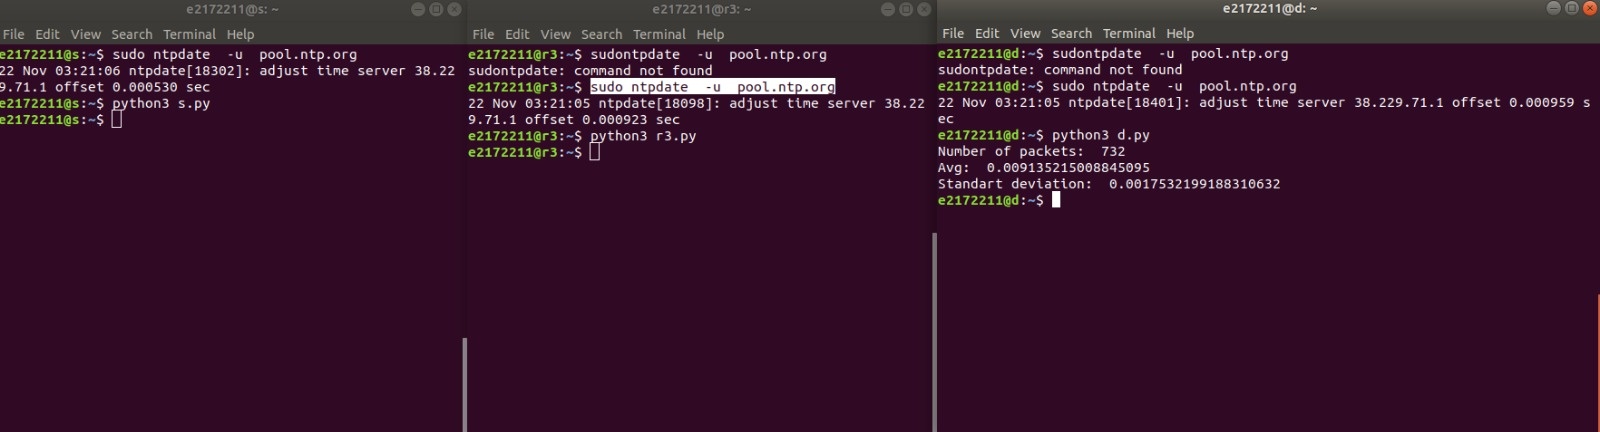
\includegraphics[width=9cm]{bibliography/delay_0.jpeg}
    \caption{End-to-end delay without any network emulation delay}
    \label{fig:delay_0}
\end{figure}

\begin{figure}[htp]
    \centering
    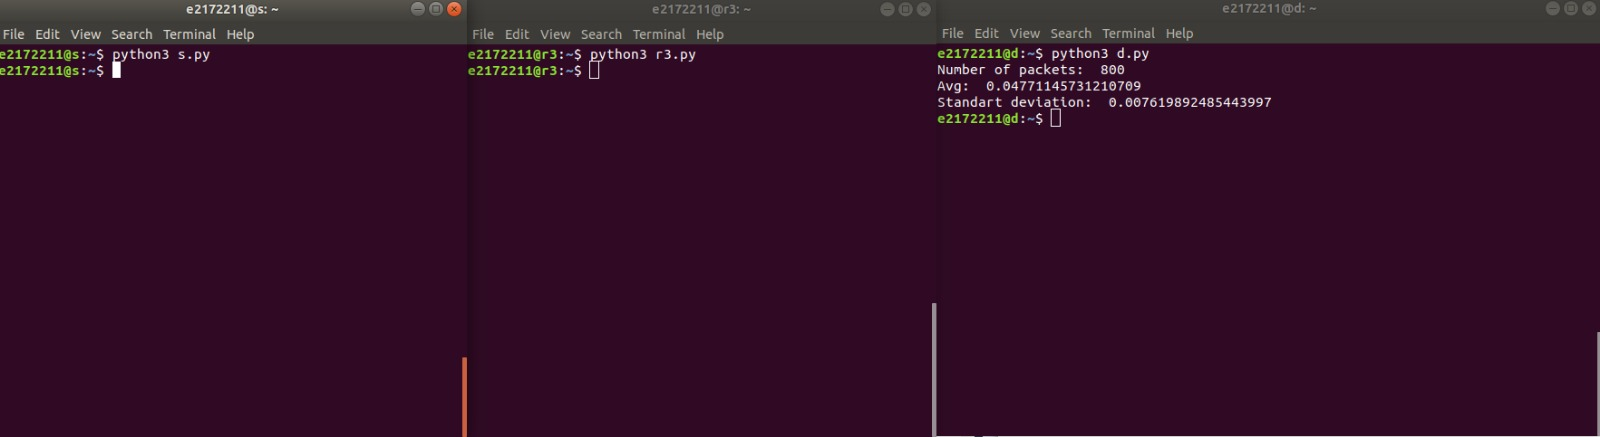
\includegraphics[width=9cm]{bibliography/delay_20.jpeg}
    \caption{End-to-end delay with 20 ms +- 5 ms network emulation delay}
    \label{fig:delay_20}
\end{figure}

\begin{figure}[htp]
    \centering
    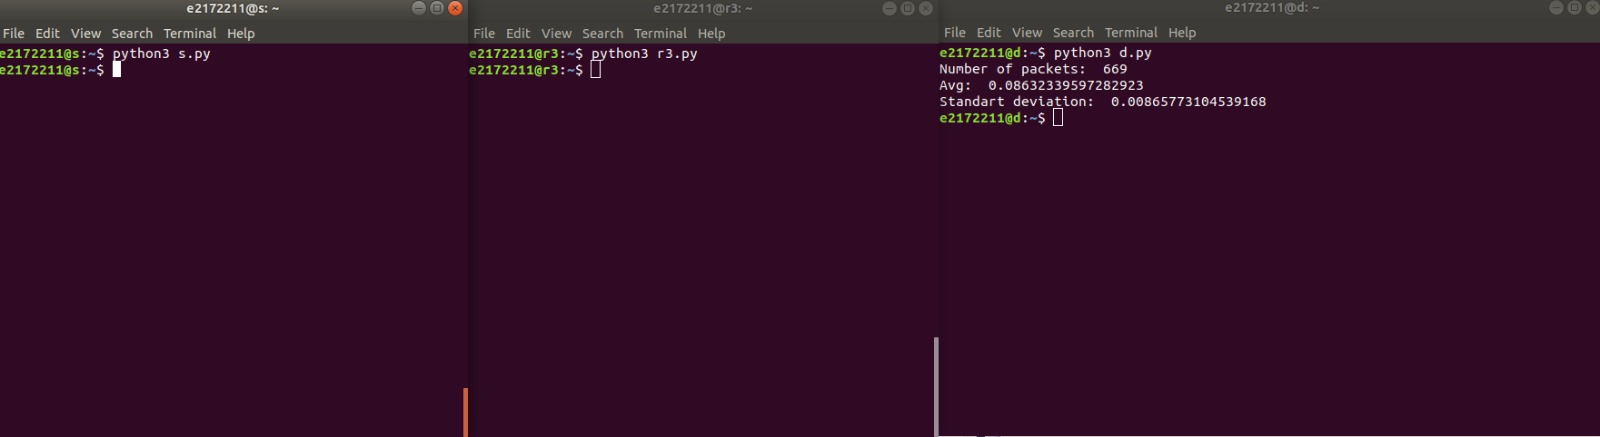
\includegraphics[width=9cm]{bibliography/delay_40.jpeg}
    \caption{End-to-end delay with 40 ms +- 5 ms network emulation delay}
    \label{fig:delay_40}
\end{figure}

\begin{figure}[htp]
    \centering
    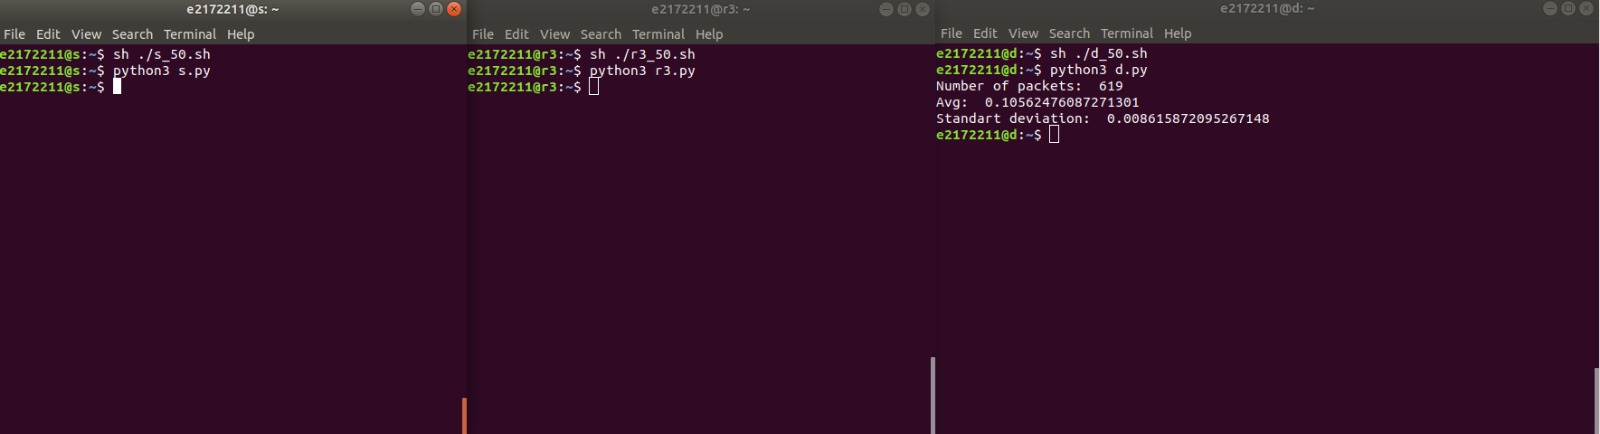
\includegraphics[width=9cm]{bibliography/delay_50.jpeg}
    \caption{End-to-end delay with 50 ms +- 5 ms network emulation delay}
    \label{fig:delay_50}
\end{figure} 

For the plot of the experiment, we needed to find margin of errors. To find them, we used the following formula: \\

$e = z * \dfrac{\sigma}{\sqrt{n}}$ \\

Here, $e$ is the margin of error, $\sigma$ is the standard deviation of end-to-end delays, and $n$ is the number of packets that had been sent. Since we use 95\% confidence interval, $z$ value is $1.96$. The calculated number of packets, standard deviations and margin of errors can be seen from Figure 6. \\

\begin{figure}[htp]
    \centering
    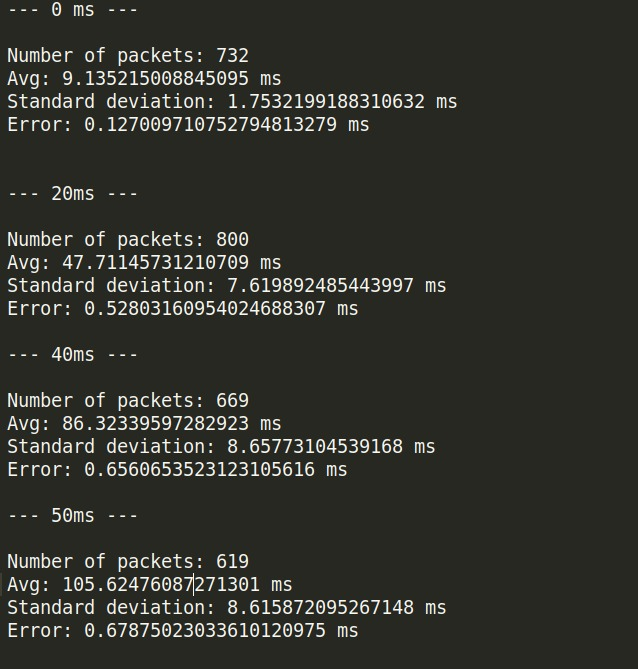
\includegraphics[width=9cm]{bibliography/values.jpeg}
    \caption{Calculated values from experiments}
    \label{fig:values}
\end{figure}




We plotted the graph with respect to those values by using GNU Octave, and it can be seen from Figure 7. \\ \\ \\ \\

We got almost purely linear graph. It makes sense because when we increase emulated network delay, end-to-end delay also increases. The emulated network delay and end-to-end delay are directly proportional. When we adds network emulated delay to both links on the path (s-r3 and r3-d), it is directly added to the end-to-end delay.

\begin{figure}[htp]
    \centering
    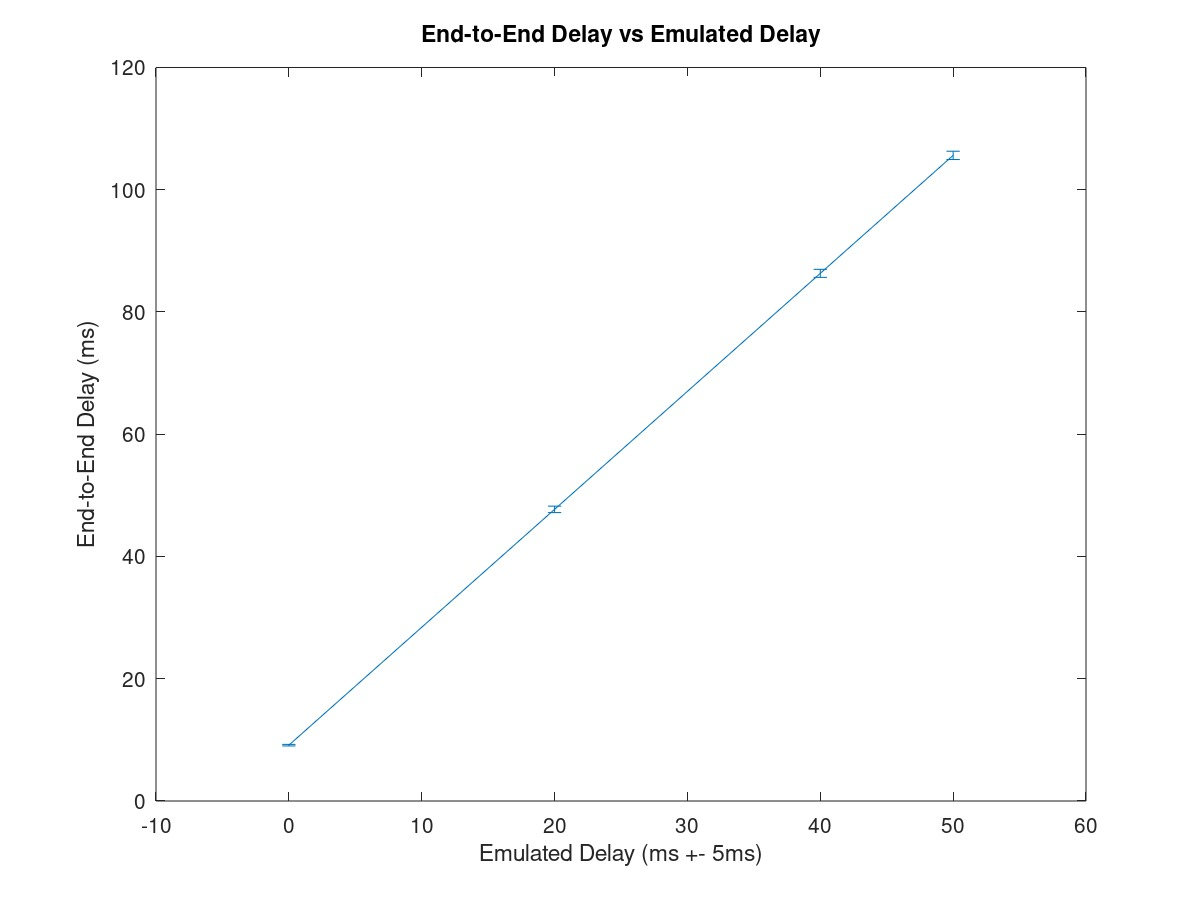
\includegraphics[width=9cm]{bibliography/emulated_vs_end-to-end.jpeg}
    \caption{Emulated network delay vs end-to-end delay}
    \label{fig:graph}
\end{figure} 

\section{Reference}
Kurose, J. F., \& Ross, K. W. (2017). Computer networking: a top-down approach. Pearson.


\end{document}
